\section{Methods}

Construction links protocol evidence to economic interpretation before defining common analytical fields. Figure~\ref{fig:oracle_dgp} summarizes source registration, native decoding, lifecycle reconstruction and harmonization. Unresolved identities, open lifecycles and unobservable outcomes remain explicit. The common schema supports comparison while preserving protocol-specific meanings.

\begin{figure}[!htbp]
\centering
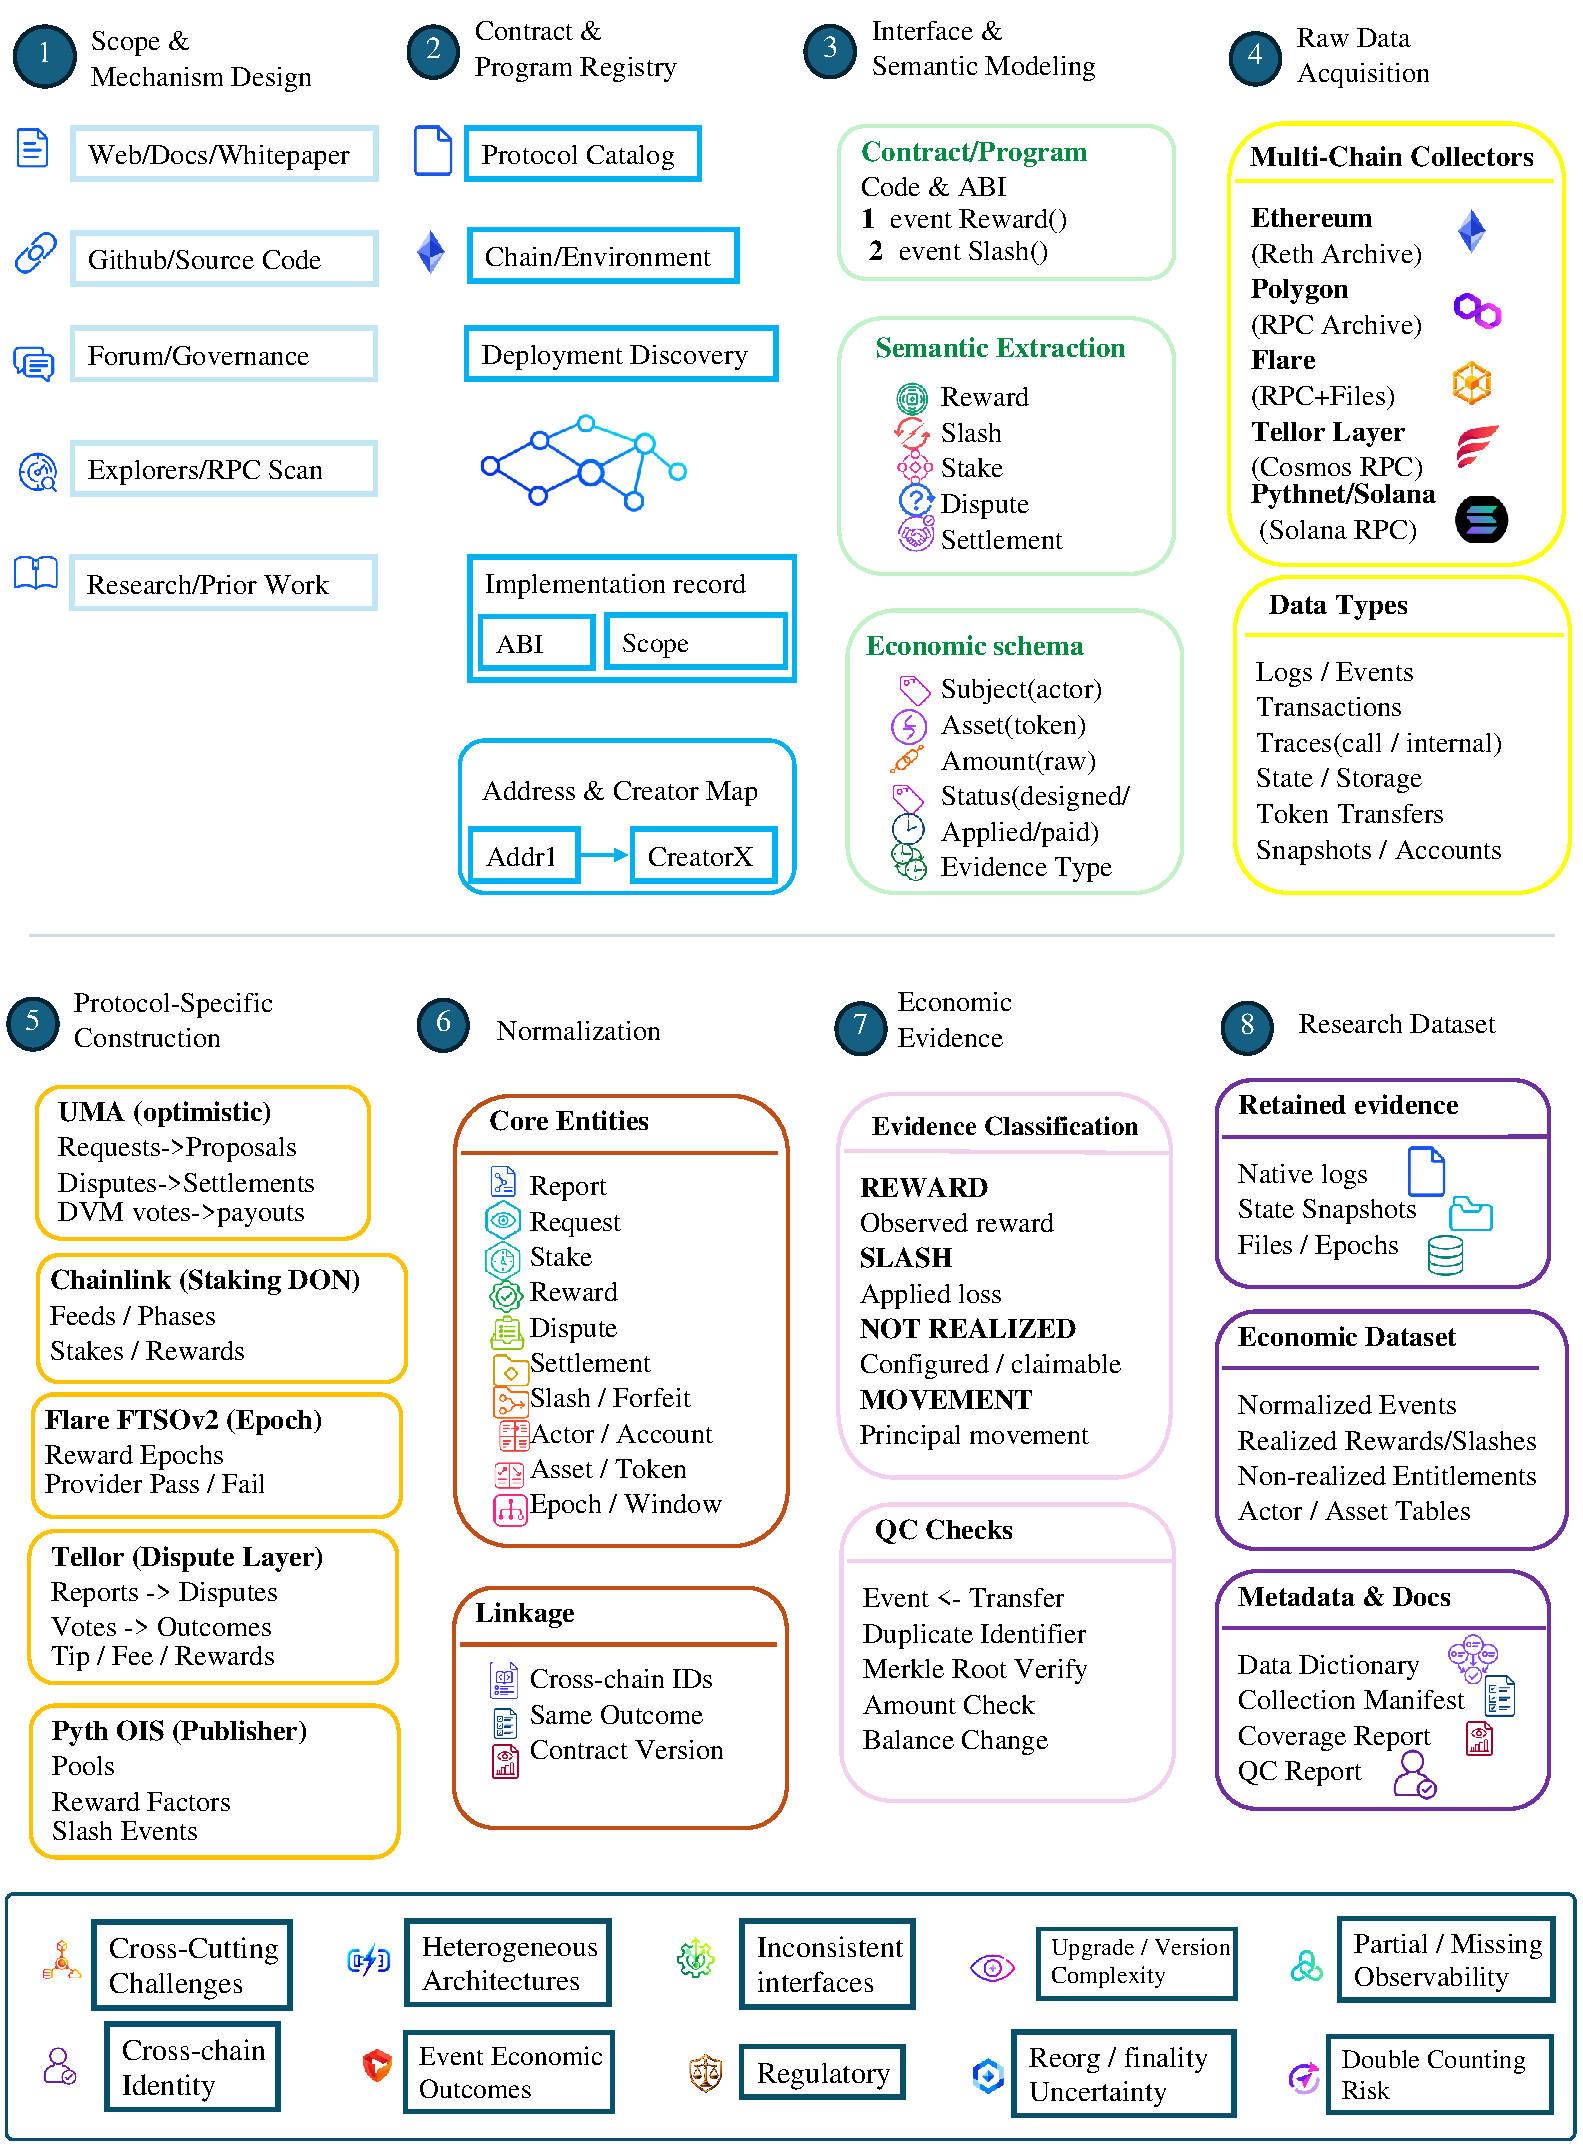
\includegraphics[width=0.99\linewidth]{figures/overview_restored.pdf}
\caption{Construction and validation workflow. Stages 1--4 register sources, define native semantics and acquire evidence; stages 5--8 reconstruct supported lifecycles and economic states for analysis and documentation. The lower strip lists measurement challenges. Checks require evidence; protocol decisions do not establish external truth.}
\label{fig:oracle_dgp}
\end{figure}

\subsection{Scope, selection and historical boundaries}

The discovery registry contains 56 oracle or related mechanism categories and 366 protocol--oracle relationships. It supports source discovery and ecosystem description, not probability sampling. Eight branches are selected for their economic mechanisms, identifiable historical records and scope for reconstruction. Each branch denotes a specified mechanism and implementation, including the chain roles observed in its records.

UMA, Chainlink, Tellor, Flare FTSOv2 and Pyth provide five detailed native panels. Chronicle, RedStone Push and DIA add narrower observations of challenge, update delivery and staking activities. Panel breadth implies neither complete histories nor equivalent variables or protocol quality. Only registered versions and services are included. Table~\ref{tab:protocol_sources} summarizes branch scope; Appendix~\ref{app:scope} lists sources and exclusions.

Chain roles are distinguished by function. A verification or adjudication chain records the relevant acceptance or dispute-resolution process; an economic settlement chain records the associated payment or applied balance change; and a delivery chain records provision of the oracle output to a consuming application. A single network may serve several roles. In the linked UMA disputes studied here, Polygon hosts the OOv2 lifecycle and observed local settlement flows, whereas Ethereum hosts VotingV2 adjudication. Linking these records establishes a relationship between protocol objects and does not, by itself, establish a cross-chain token transfer. The eight branches consequently do not denote eight independent blockchains.

The common upper observation cutoff is 30 June 2026 at 23:59:59 UTC. Table-level temporal support is documented separately from protocol history in Appendix~\ref{app:temporal}. The temporal register identifies deployment-bound scans, implementation changes, retained-history limits and cohort restrictions without treating a first event as a deployment date. Lower boundaries vary with deployment, implementation changes, historical source availability and collection limits. Project founding dates, production-service launches, deployment boundaries, scanned intervals and first observed events are distinct quantities. An interval between the first and last retained events does not establish uninterrupted observation. Transaction histories and retained state panels may also have different temporal support, as in the Pyth OIS branch. Historical interpretation requires an implementation applicable to the observation; unresolved source bindings and acquisition gaps remain limitations. Current protocol documentation supplies architectural context~\cite{uma2026,chainlinkstaking2026,tellorDisputes2026,flareFTSO2026,pythOIS2026,chronicleDocs2026,redstoneDocs2026,diaDocs2026}, while Appendix~\ref{app:scope} distinguishes that context from retained historical evidence.

\begin{table}[!htbp]
\centering\tabstyle[registrytint]
\caption{Measurement roles, implementation scope and historical boundaries of the eight oracle branches. Coverage refers to registered sources, not all services of a protocol. The upper cutoff is 30 June 2026, 23:59:59 UTC. Appendix~\ref{app:scope} separates deployment, scanning and retained-event boundaries.}
\label{tab:protocol_sources}
\begin{tabularx}{\linewidth}{@{}L{0.105\linewidth} L{0.22\linewidth} L{0.255\linewidth} Y@{}}
\toprule\tablehead
\textbf{Branch} & \textbf{Implementation and chain} & \textbf{Registered coverage} & \textbf{Measurement role and main exclusion} \\
\midrule
UMA & Ethereum VotingV2; Polygon OOv2 and adapters & DVM blocks 16,697,232--25,433,938; Polygon contract-specific starts through 89,439,336 & Proposals, disputes, adjudication and settlement. Other UMA versions and deployments are outside the registered scope. \\
Chainlink & Ethereum Staking v0.2; ETH/USD proxy and feed phases & Staking from block 18,572,190; registered sources through 25,433,938 & Staking economics and selected feed updates. Other feeds, networks and services are excluded. \\
Tellor & \texttt{tellor-1} modules, ABCI events and block results & Heights 1--19,890,860; first report at height 317 & Reports, disputes, votes, payments and restrictions. Legacy Ethereum Tellor is excluded. \\
Flare FTSOv2 & Flare RewardManager, VoterRegistry and reward artifacts & Closed reward epochs 228--410; cutoff block 64,054,789 & Entitlements, provider conditions and claims. Table coverage differs; aggregate claims may resist attribution. \\
Pyth & Solana OIS transactions and retained Pythnet-derived inputs & Transaction archive from 11 September 2024; 49 retained closed state epochs & Publisher--epoch states, staking and transfers. State coverage is shorter; other products and delivery networks are excluded. \\
\midrule
Chronicle & Registered Ethereum validator and challenge contracts & Registered log scan 0--25,433,938; deployment dates are separate & Reports, challenges and challenge rewards. Rewards are not a complete publisher-compensation ledger. \\
RedStone Push & Registered Ethereum Push adapters and feeds & Registered log scan 0--25,433,938; deployment dates are separate & Signed publication and Push updates. Other delivery modes and full AVS economics are excluded. \\
DIA & Registered Lasernet staking contracts & Deployment block 3,874,186 through cutoff 31,302,665 & Withdrawals, returned principal and rewards. This is not a complete price-production or delivery audit. \\
\bottomrule
\end{tabularx}
\end{table}


\subsection{Source acquisition and native decoding}

For each branch, a source register identifies the network, contract or program, implementation, collection interval and retrieval interface. EVM-compatible branches use historical logs, supplemented where necessary by transactions, receipts, block metadata and token-transfer evidence. ERC-20 transfers are retained when they help separate principal, fees and rewards from a settlement event. Tellor instead combines tellor-1 module state, ABCI events and block results; multiple reports within one block produce a one-to-many expansion into 82,866,640 report observations. Pyth evidence is located by Solana transaction signatures and outer or inner instruction positions. Flare combines on-chain records with official reward-calculation artifacts, preserving the distinction between entitlement and claim.

Decoding follows the registered version and cutoff. Polygon UMA has 626,578 raw records, including five unknown event topics retained only in the raw collection. Chainlink staking has 175,015 collected logs, yielding 174,890 decoded events and 125 unclassified records. Unclassified records do not indicate absent economic behavior. Tables retain native keys, integer amounts, asset identifiers and decimal precision.

\subsection{Lifecycle reconstruction and cross-chain linkage}

Decoded records are joined where the native mechanism identifies a relationship between successive states. UMA requests link proposals, disputes, DVM adjudication and settlement through reconstructed request identifiers. For requester $r$, identifier $i$, timestamp $t$ and ancillary data $a$, the identifier is
\begin{equation}
 q = \operatorname{Keccak256}\!\left(\operatorname{pack}(r,i,t,a)\right),
 \label{eq:requestid}
\end{equation}
where $\operatorname{pack}$ denotes the protocol's packed ABI encoding. The reconstructed OOV2 panel contains 42,676 request rounds: 41,826 settle by the cutoff and 850 remain open. Other mechanisms require different objects. For example, 46,723 retained Chainlink ETH/USD answer updates define 46,722 adjacent service windows, and 13 Tellor jail events are paired with 13 release events to reconstruct reporter restrictions.

Cross-chain identity is established through version-aware ancillary-data transformations and native request construction. A UMA link receives Grade A only when the registered bridge or adapter rule identifies one unique DVM request. Of 835 attempted links, 832 meet this deterministic definition and three remain unmatched. The grade describes the identity of a reconstructed object; it does not certify the factual correctness of the oracle's decision. Retaining unmatched and unfinished objects prevents the apparent completeness of an analytical table from replacing evidence about the underlying process. The worked case links request, proposal, dispute, DVM resolution and Polygon settlement. Each endpoint is located by its chain, transaction and log position. The retained evidence supports the object linkage and elapsed intervals; intermediate relay operations are represented separately where their transactions are not retained.

\subsection{Economic states and settlement accounting}

An economic observation is classified by its state and evidentiary basis. Table~\ref{tab:economic_states} distinguishes configured incentives, accrued rewards or penalties, claimable entitlements, realized payments, applied losses, principal, refunds and fees. The distinctions are protocol-specific. UMA challenge status requires native challenge evidence, and settlement is not inferred merely from a transfer-like event. Tellor SUPPORT outcomes refer to acceptance of the challenge and rejection of the challenged report. Negative DVM accruals remain distinct from an observed reduction in staked principal. Pyth reward rates are not token reward amounts, and Flare participation restrictions are not automatically monetary losses.

UMA settlement provides a concrete accounting example. Let $B$ be the effective bond, $F$ the final fee and $R$ the configured reward, all measured in the smallest integer unit of the same asset. Posted principal is $P=B+F$. For disputed requests, the identifiable winner component is $W=B-\lfloor B/2\rfloor$, while the protocol component is $F_{\mathrm{protocol}}=\lfloor B/2\rfloor+F$. Expected gross payouts follow the registered contract and adapter rules:
\begin{align}
 G_{\mathrm{undisputed}} &= B+F+R, \nonumber\\
 G_{\mathrm{disputed}} &= B+F+W+R_{\mathrm{settlement}}.
 \label{eq:payout}
\end{align}
Here $R_{\mathrm{settlement}}$ is the reward attributable to settlement under the applicable adapter; refunds and rollovers are not automatically participant income. Exact integer reconciliation requires $\Delta_{\mathrm{payout}}=G_{\mathrm{actual}}-G_{\mathrm{expected}}=0$.

In Section~\ref{sec:case}, a 1,000-unit payout comprises 750 in principal and 250 in gain before costs. A configured five-unit reward is refunded or rolled over as observed. Net profit requires cost data. UMA settlements are checked against token movements, Chainlink separates transfer-requiring events from accounting adjustments, and Flare reconciliation retains only components supported by the claim evidence.

\begin{table}[!htbp]
\centering\tabstyle[economictint]
\caption{Economic states distinguished in reconstruction. Each classification requires the evidence specified by the originating protocol. A lifecycle need not expose every state.}
\label{tab:economic_states}
\begin{tabularx}{\linewidth}{@{}L{0.20\linewidth} L{0.33\linewidth} Y@{}}
\toprule\tablehead
\thcell{clock}{State} & \thcell{coin}{Economic meaning} & \thcell{compare}{Interpretation rule} \\
\midrule
Configured incentive & Reward specified in protocol parameters & A design parameter; not automatically participant income. \\
Accrued reward or penalty & Calculated entitlement or liability & Distinct from subsequent payment or application; counting both may duplicate one change. \\
Claimable entitlement & Amount eligible for a claim & An unclaimed entitlement is not a zero payment or a realized transfer. \\
Paid reward & Observed transfer or realized protocol credit & Realized only when qualifying cash-flow or state evidence is present. \\
Applied slash & Reduction applied to a participant's balance or principal & Requires observed application, beyond a penalty calculation or accrual. \\
Principal deposit or return & Capital posted and subsequently recovered & Kept separate from rewards and fees; returned capital is not profit. \\
Refund or rollover & Incentive returned or carried to another state & Not attributed to the current participant without supporting evidence. \\
Protocol fee & Amount charged or retained under protocol rules & Separated from participant reward and principal. \\
\bottomrule
\end{tabularx}
\end{table}


\subsection{Harmonization, missingness and documentation}

Common fields retain protocol, unit, role, actor or beneficiary, lifecycle identity, time, asset, economic stage, source and evidence status. The accountability layer contains 105,588,120 typed observations; the economic layer contains 22,723,389 components, including 19,275,854 meeting branch-specific payment or applied-state criteria. These overlapping layers describe the same underlying processes at different levels.

Timestamp availability differs from coverage: a valid clock on every retained row does not prove complete collection, and a missing clock does not imply an absent event. Epoch and snapshot clocks remain distinct from canonical event time. Missing values can indicate inapplicability, unexposed quantities, incomplete collection, decoding problems or unfinished lifecycles. They are not automatically zero. Where supported, schemas distinguish complete, partial, verified-zero, unknown, unavailable and not-applicable coverage; right censoring is recorded separately. Deduplication uses native keys and preserves legitimate multiplicity across representations and economic components. Table~\ref{tab:processing_pipeline} summarizes these operations.

\begin{table}[!htbp]
\centering\tabstyle[acquisitiontint]
\caption{Processing operations and their outputs. Rows describe transformations rather than statistically independent populations: operations may expand, aggregate, join or decompose their inputs.}
\label{tab:processing_pipeline}
\begin{tabularx}{\linewidth}{@{}L{0.21\linewidth} L{0.39\linewidth} Y@{}}
\toprule\tablehead
\thcell{clock}{Operation} & \thcell{document}{Input and rule} & \thcell{data}{Output} \\
\midrule
Source registration & Network, contract or program, historical version, interval and interface & Branch-specific collection specification. \\
Acquisition and qualification & Logs, transactions, receipts, block or module state, signatures and protocol artifacts; cutoff and decoding rules & Qualified source records, with unresolved decoding outcomes retained. \\
Native decoding & Protocol event and state definitions; integer amounts and native keys & Protocol-native tables. \\
Lifecycle reconstruction & Request, dispute, claim, epoch or other native object relationships & Supported lifecycle objects and open cases. \\
Cross-chain linkage & Version-specific identifier and ancillary-data transformations & Deterministic matches, link grades and unmatched cases. \\
Economic-state mapping & Native lifecycle and accounting evidence & Configured, accrued, claimable, paid, applied, returned, refunded and fee components. \\
Funds-flow reconciliation & Expected quantities against observed transfers or applied state changes & Realization flags and accounting differences. \\
Harmonization & Shared concepts with native units and source links retained & 105,588,120 typed accountability observations. \\
Realization filtering & Protocol-specific evidence conditions applied to 22,723,389 economic components & 19,275,854 qualifying realized components. \\
Documentation & Dictionaries, schemas, coverage information, source registers and validation results & Interpretable data and reconstruction materials. \\
\bottomrule
\end{tabularx}
\end{table}


Documentation records native identifiers, source registers, input inventories, schemas, variable definitions and validation rules. Quality controls assess selected key relationships, lifecycle orderings, cutoff conditions, economic identities and deterministic links. The accompanying artifacts identify the tested populations and the evidence available for reconstruction. Their traceability supports inspection of specific mappings, while leaving incomplete historical acquisition and unresolved source ancestry visible.

\subsection{Temporal harmonization}
\label{sec:temporal}

Native timestamps are expressed in UTC while retaining their original values and precision. Each time field is documented by its source, unit and role in the protocol. The field \codefield{event_time_utc} identifies when an event was recorded or executed. Request-reference timestamps, oracle payload times and scheduled deadlines are represented separately because they can refer to a different point in the lifecycle. Records sharing a timestamp retain their native block, transaction, log or instruction order.

Unix-second and millisecond values are converted without rounding. Textual timestamps are interpreted using their recorded timezone; timezone-naive values are treated as UTC where this convention is established by the source. Missing EVM event times are recovered only when another retained record identifies the timestamp of the same block on the same chain. Conflicting matches are rejected and unmatched observations remain undated. The provenance of recovered timestamps is recorded with the data.

Epoch observations retain their start and end times as half-open intervals $[a_e,b_e)$. Payment, snapshot and retrieval times describe separate events and are stored independently. In particular, an epoch-end label does not establish when a reward became claimable or was paid. Historical state recovered from a later snapshot also requires care when assessing information available at a past decision time.

Daily windows begin at midnight UTC, and weekly windows run from Monday to the following Monday. Epoch totals remain attached to their native support intervals. Daily aggregation therefore requires an event-level measure or an explicit allocation rule, together with evidence that the relevant period was observed. Appendix~\ref{app:temporal} describes the native clocks and temporal limitations of each branch.


\subsection{UMA prediction-task construction}
\label{sec:prediction}

The prediction task asks whether UMA's eventual resolution differs from the proposed price. Each observation is one request, and the decision time $T_0$ is the proposal event. For proposed price $p_i$ and resolved price $z_i$, the label is $Y_i=\mathbf{1}\{z_i\ne p_i\}$. Native values are compared as integers. Indeterminate and early-expiration values retain their own classes; neither is recoded as a binary answer.

Eligibility requires a challenged request, a unique deterministic DVM link, consistent resolution values and a reconciled settlement transfer. Because selection is retrospective, the task concerns adjudication among selected disputes, not challenge risk for new requests. Challenge, resolution and settlement fields supply outcome evidence and are excluded from predictive inputs.

The sixteen candidate features describe incentives, timing, ancillary-data length, participant history and adapter identity. Proposer and requester histories are calculated separately from requests settled before the current proposal in native execution order. Rates are missing without prior settlements. Proposal latency begins at the request event; liveness ends at expiry. Parameter-derived features require evidence of availability at $T_0$ and carry a separate status. Appendix~\ref{app:prediction} defines the features and their information boundary.

\subsection{Daily economic measurements}
\label{sec:daily}

Daily observations use midnight-to-midnight UTC intervals and retain branch, implementation, actor role, asset, unit and economic stage. Feasibility distinguishes derivable measures, additional acquisition requirements, inapplicable quantities and unresolved cases. Appendix~\ref{app:daily} defines aggregation and denominators.

Payments enter the daily product only under the relevant realization rule. UMA rewards are separated from returned principal and forfeited bonds. VotingV2 net stake applications retain their own economic stage and are not added to request-level accruals; Tellor withdrawals into stake and Pyth transfers to stake custody retain those destinations. Flare fee burns are excluded from participant payments. Chainlink claims require a matched transfer and an execution timestamp. An unobserved day is left unfilled, and totals over retained records are not presented as complete protocol totals.

Participation measures count addresses within a named role. Reward concentration is calculated among recipients with positive observed payments, separately by asset and economic stage. For completed UMA requests, delay runs from the request event to settlement, and escrow exposure integrates observed balances between successive transfers. Only unambiguous closed request flows with nonnegative intermediate balances are included; the measure includes funded rewards while held and does not represent unresolved capital obligations. Flare signing weights and thresholds are retained on their native epoch intervals; they are not interpreted as daily payments or token collateral.
